\documentclass[../TM3-UltraDoc.tex]{subfiles}
\begin{document}
	\section*{7) Planar graphs}
	\addcontentsline{toc}{section}{7) Planar graphs}
	% Your content here
	\textbf{Планарный граф (Planar graph)} - граф, который можно представить на плоскости так, чтобы никакие 2 ребра не пересекались (кроме общих концов(вершин))\\
	\\
	\textit{Примечание (спизжено с исагиллы) - есть еще плоские графы (plane graph), это те графы которые не просто можно, а уже изображены на плоскости, без пересечения ребер}\\
	\small
	\begin{tcolorbox}[colframe=gray!50!black, left=5pt, right=5pt, top=5pt, bottom=5pt, boxrule=1pt, colback=gray!10!white, title=\text{Ладно, теперь поговорим серьезно}]
		\begin {itemize}
		\item Существуют признаки-теоремы планарности графа
		\item 2 точные теоремы, и значат по сути одно и тоже - теорема Куратовского и теорема Вагнера
		\item Теорема Куратовского:\\
		Конечный граф является планарныым, тогда и только тогда, когда не соджержит подграф, являющийся подразделением (полного графа на 5 вершинах ($K_5$) или полного двудольного графа 3,3 ($K_{3,3}$))\\
		\textit{сформулированно по-ублюдски, теорема Вагнера мне нравится куда больше}
		\item Теорема Вагнера:
		Конечный граф является планарным, тогда и только тогда, когда не содержит $K_5$ или $K_{3,3}$ как минор.
		\item коротенький экскурс в терминологию происходящего:
			\begin{itemize}
				\item подграф - граф, который можно получить путем удаления вершин и ребер исходного графа
				\item подразделение (subdivision, возможно не самый лучший перевод, ну ладно) граф получаемый делением ребра (ребер) на несколько, путем добавления вершин в середину (возможно 0 раз, так что сам граф является своим собственным подразделением)
				\item минор - граф, который можно получить путем удаления вершин, удаления ребер, сокращения ребер исходного графа
			\end{itemize}
			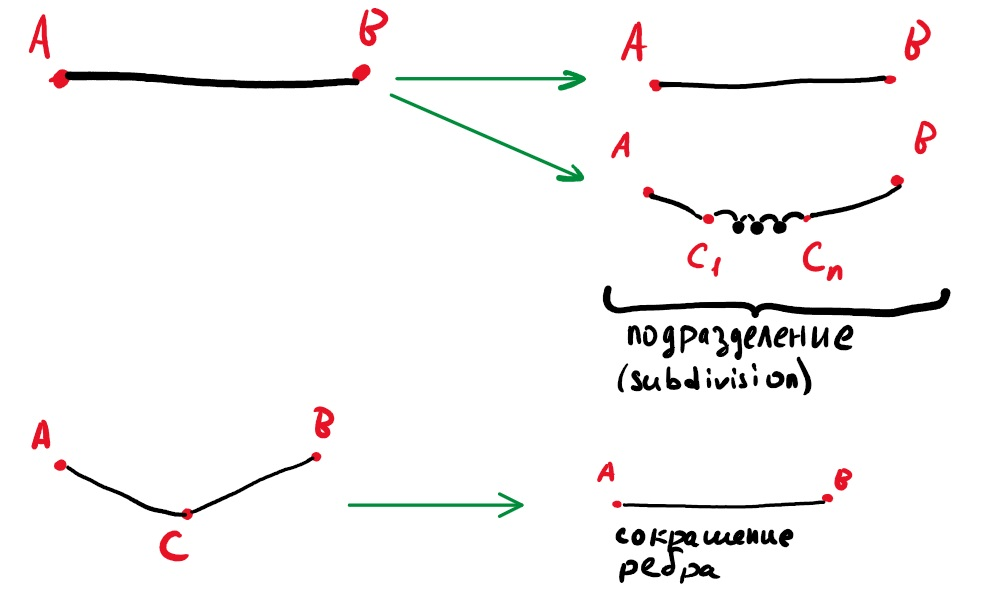
\includegraphics[width = 0.8\textwidth]{7.1}
		\item ну и некоторые менее точные признаки:
			\begin{itemize}
				\item \(|E| < 3|V| - 6\)
				\item \(|E| < 2|V| - 4\) (если нет циклов длинной 3)
				\item \(f < 2|V| - 4\) ($f$ - кол-во "поверхностей")
				\item и много много много других...\\
				\href{https://en.wikipedia.org/wiki/Planar_graph}{Вот статья на википедии}
			\end{itemize}
	\end{itemize}
	\end{tcolorbox}
	\normalsize
\end{document}